\chapter{Task Resolution}
This chapter will describe all the tasks handled in this sprint in varying degrees of detail depending on the significance and uniqueness of the solution.

\section{Update Dependencies}
In the current state of the Giraf project the individual sub-project, which are applications or libraries for Android, uses a series of common libraries made for the Giraf project.
Their dependencies are not all updated to use the newest version, this might introduce bugs which have already been fixed.
For this reason the first order of business, should be updating these such that this years Giraf project will start with the fewest issues regarding the dependencies. 
We have taken three tasks which relates to this, namely upgrading the dependencies of the applications Sequence and the two libraries Sequence-Viewer and Picto Search.
We took these as they all had the same versions in common to be upgraded, they are:
\begin{itemize}
    \item \texttt{localDB} from version 5.1.2 - 5.1.5
    \item \texttt{meta-database} from version 3.2.0 - 3.2.3
    \item \texttt{oasisLib} from version 7.2.0 - 9.0.2
\end{itemize}
The first two of these \texttt{localDB} and \texttt{meta-database} only have their patch-number updated, this should indicate a bug-fix or small internal corrections, as such they should not introduce any issues in upgrading. 
\texttt{localDB} is a library which is used to store information in a local database, most of this data is received when the Giraf Launcher is opened the first time. 
This is to reduce the inconvenience of having either a slow or no internet connection, however it also introduces some problems regarding keeping the remote database and the local one in sync. 
\texttt{meta-database} is used to create the \texttt{localDB}, the changes therein does not affect any of the applications we are tasked with upgrading. 

\texttt{oasisLib} is the connection from the tablet to the remote database.
In the upgrade from 7.2.0 to 9.0.2, some of the methods used in the applications and libraries to be upgrades was deprecated, and subsequently removed. 
One such method is the one which is responsible for loading pictograms.
All uses of this has to be replaced with the new method of loading pictograms. 
This now uses a helper, \texttt{pictogramHelper}, which has replaced the methods used directly on the model. 

\begin{description}
    \item[Sequence-Viewer] \hfill \\
    The Sequence-Viewer used the model directly to get an image, since this was deprecated when updating \texttt{oasisLib}.
    This method is used to replace a pictogram in a view after selecting an option from a multiple choice. 
    To resolve this issue the line shown in \myref{lst:dep-sv-prev} were changed to \myref{lst:dep-sv-upd}. 
    \begin{figure}
        \begin{lstlisting}[language=java, caption={Sequence-Viewer with deprecated method call. }, label=lst:dep-sv-prev]
/* [...] */
pictogram.setImage(
    helper.pictogramHelper.getById(id).getImage());
/* [...] */
        \end{lstlisting}
    \end{figure}
    \begin{figure}
        \begin{lstlisting}[language=java, caption={Sequence-Viewer replacement code. }, label=lst:dep-sv-upd]
/* [...] */
// The helper setImage function no longer acquires the pictogram name and causes null exception error
// This check for null and queries the name by ID to get name
if(helper.pictogramHelper.getById(id).getName() == null) {
    pictogram.setName("pictogram_name");
}
else {
    pictogram.setName(
        helper.pictogramHelper.getById(id).getName());
}
helper.pictogramHelper.setImage(pictogram, 
    helper.pictogramHelper.getImage(
        helper.pictogramHelper.getById(id)));
/* [...] */
        \end{lstlisting}
    \end{figure}
    Additonally a null-check have been added to assure that a name, locally, is never set to \texttt{null}, as this can cause issues in other methods which assumes that every pictogram has a name. 
    After resolving these issues the application was tested and it worked as the previous stable version did. 
    \item[Sequence] \hfill \\
    After upgrading to the newest versions of the libraries mentioned above Sequence was unable to build. 
    This was caused by the usage of a deprecated method. 
    The solution to this issue was fixed by changing a single line to use the correct replacement for the deprecated method.
    The previous code is show in \myref{lst:dep-seq-prev}, and the fixed code is shown in \myref{lst:dep-seq-upd}.
    \begin{figure}
        \begin{lstlisting}[language=java, caption={Sequence with deprecated method call. }, label=lst:dep-seq-prev]
/* [...] */
pictogram.setImageBitmap(
    helper.pictogramHelper.getById(id).getImage());
/* [...] */
        \end{lstlisting}
    \end{figure}
    \begin{figure}
        \begin{lstlisting}[language=java, caption={Sequence using the replacement code. }, label=lst:dep-seq-upd]
/* [...] */
pictogram.setImageBitmap(
    helper.pictogramHelper.getImage(
        helper.pictogramHelper.getById(id)));
/* [...] */
        \end{lstlisting}
    \end{figure}
    The line in question is responsible for loading the pictograms from the database into the application. 
    Previously the model had been used directly however in \texttt{oasisLib} 9.0.2 this is unsupported.
    The method call \texttt{.getById(id)} returns a pictogram object and on that object the \texttt{.getImage()} method is called.
    The reason for it being unsupported is that the model should not be used directly, but rather the helper should be used.
    In other words the \texttt{.getImage()} method have been removed from the pictogram model class in \texttt{oasisLib} 9.0.2. 
    After this replacement was made then we informally verified that the application worked identically to the previous version with the old dependences.
    Then a diff was submitted, approved and landed in the master branch, following the work flow of the multi-project. 
\end{description}

\subsection{Wiki Migration}
We have the area of responsibility ``Documentation and Wiki'', part of this is ensuring that the information in the Redmine wiki made by the previous GIRAF students is kept since we will depreciate Redmine in favor of Phabricator.
On the Redmine wiki there is a lot of useful information, some of it might be outdated, but most is still useful and should be kept. 

We have taken the task of starting the new wiki on Phabricator, and migrate the useful information from the Redmine wiki to it.
Part of this is to create a structure which the other members of the GIRAF project can use.
It should be noted that the wiki is only used for internal matters inside the GIRAF project.  

It is important that the front page of the wiki is easy to navigate, as this serves as the entry point and from which where all content should be found. 
The contents of the front-page is:

\begin{enumerate}[topsep=0pt,itemsep=-1ex,partopsep=1ex,parsep=1ex]
    \item Actionable Commitments
    \item Guides
    \item GIRAF Project Goals
    \item Useful Links
    \item Sprint Dates
    \item Backlog
    \item Groups and Slack Channels
    \item Wordlist
\end{enumerate}

Most of the content on the wiki are guides which helps the developers with various tasks. 
These should be easy to navigate and have titles which clearly encompass their purpose and content. 
We separate the guides made during this years GIRAF project, which are updated, from the ones made previously. 
Additionally we clearly indicate that the ones constructed previously are not up-to date with the following warning on the top of the page: ``IMPORTANT: This wiki entry has not been updated in 2016''. 

All members of the GIRAF project have access to add to and edit the wiki. 
It is the primary way to share information such as guides and overviews. 
However if this remains unmoderated then the contents of the wiki will most likely become unstructured. 
Therefore in addition the initial migration, we have setup e-mail alerts in Phabricator such that we get a notification every time someone changes the wiki.
Then we will review their additions to ensure that they are located correctly and linked to from the relevant pages etc. 
This will be an ongoing task as part of our area of responsibility.
\section{Consistent File Encoding}
\todo[inline]{TODO}
\section{Responsive Search}
\userstory{As a User I would like the Picto Search application to feel more responsive when I search for pictograms, such that I don't feel like nothing happens.}

The task is prioritised as \phigh,is estimated at 8 EP, and was created because the customers expressed concern for the reactiveness of the PictoSearch application --- it sometimes felt slow and customers said it felt like nothing was happening.
The PictoSearch application is used whenever the user needs to find a certain pictogram for other applications such as the week schedule or the sequence application.
It is a problem that the users feel like the application is slow and that it does not react quickly to what the user is doing, especially in an application used often by other applications of GIRAF.
It is important that responses from a mobile application are given within a few seconds, as mentioned in~\cite{Roto:2005:NNF:1062745.1062747}, if an application spends more than 4 seconds to load or respond then other feedback than visual should be used.
Therefore the amount of time spent waiting for the application should be reduced, such that there is no need for using other methods of feedback when the search finally returns.
According to Constantine and Lockwood in their book \enquote{Software for Use: A Practical Guide to the Models and Methods of Usage-Centered Design} \cite{DESIGNBOOK}, a design principle regarding feedback is as follows:

\begin{displayquote}
\textit{Keep users informed of actions or interpretations, changes of state or condition and errors or exceptions that are relevant and of interest to the user through clear, concise, and unambiguous language familiar to users\cite[p.~57]{DESIGNBOOK}.}
\end{displayquote}

Therefore it is decided that the Picto Search application should give visual feedback whenever an action occurs.
The application should respond to the users action more often than what it does now to increase how responsive the application feels to the user.

The current version of the PictoSearch application searches whenever the user taps the search button on either the on-screen keyboard or in the GUI of the application.
The search button is located in the middle of the screen, to the left of the search field as can be seen on \myref{fig:screenshot_startup}.

\begin{figure}[h]
    \centering
    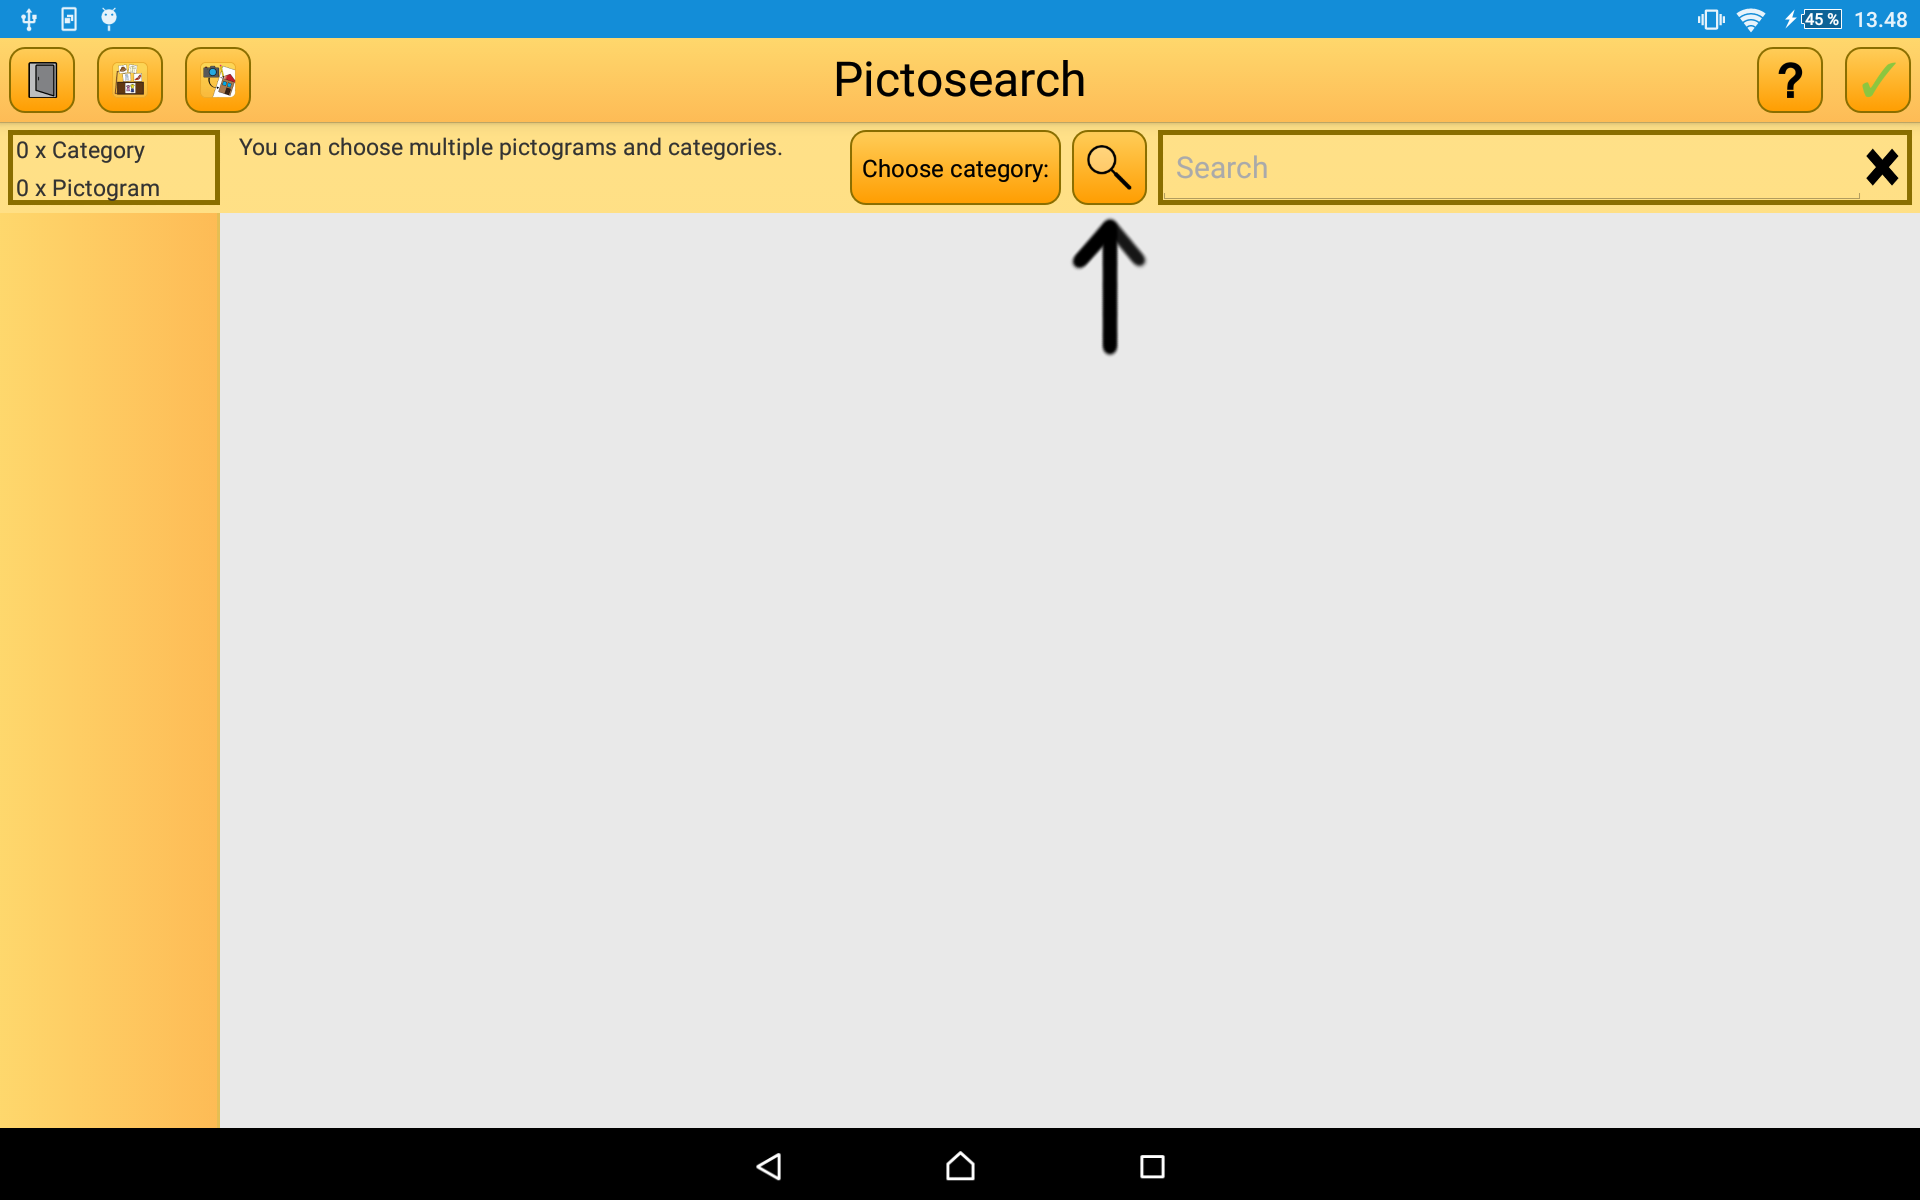
\includegraphics[width=0.8\textwidth]{figures/img/screenshots/old_startup.png}
    \caption{Screenshot of the initial view presented to the user when launching PictoSearch, with the search button highlighted.}\label{fig:screenshot_startup}
\end{figure}
\noindent
The screenshot also shows the view of the application as it is opened, completely empty with no information.

\begin{figure}[h]
    \centering
    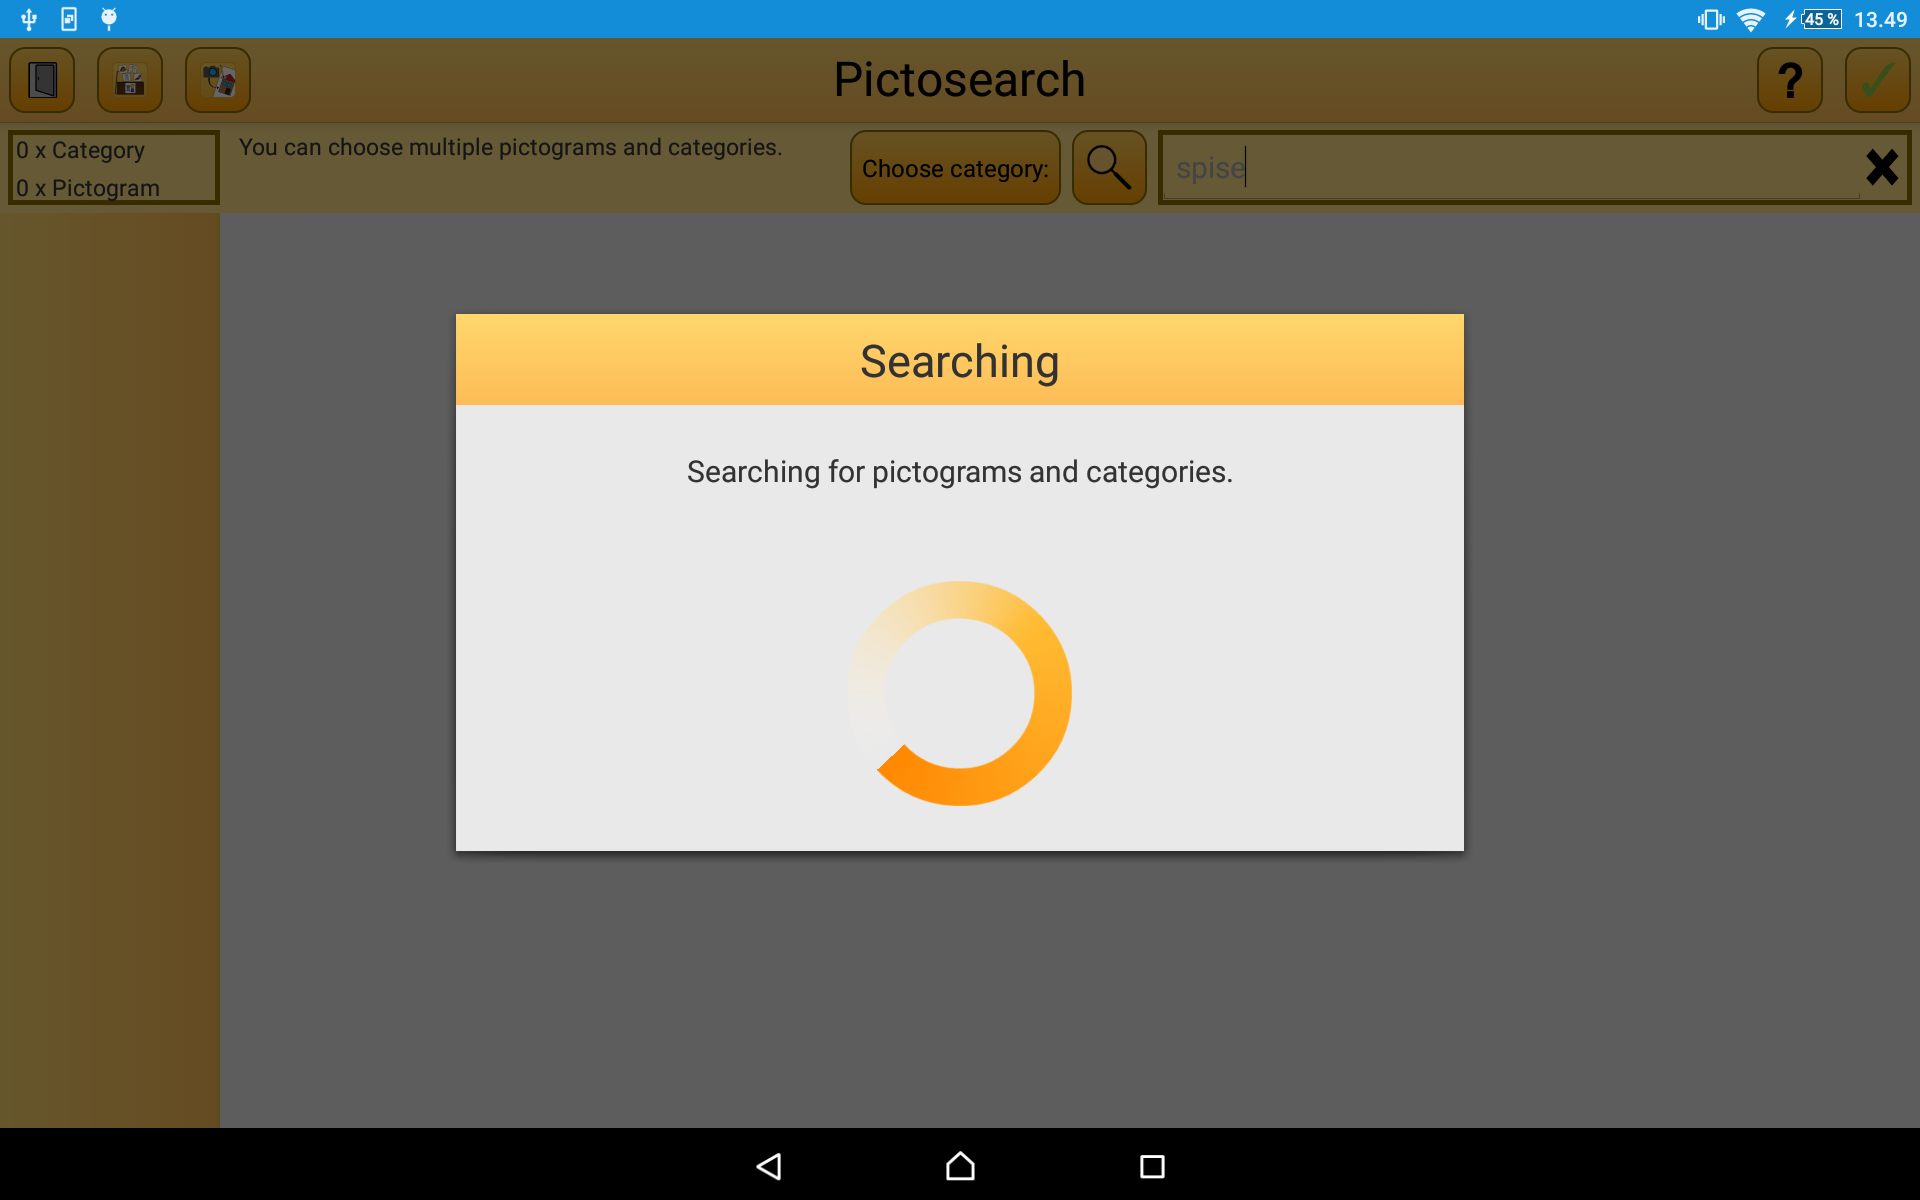
\includegraphics[width=0.8\textwidth]{figures/img/screenshots/old_dialog.png}
    \caption{Screenshot of the search spinner shown while searching in PictoSearch.}\label{fig:screenshot_searchspinner}
\end{figure}

In the new version, a search is made whenever the text in the searchfield is changed.
Instead of the big slow search spinner, which blackened out and locked the screen, shown on \myref{fig:screenshot_searchspinner}, a new smaller text message is instead displayed which tells the user that the application is searching and what is is searching for. 
The current version would also remove the on-screen keyboard when it would search, this only happens in the new version whenever the search button is pressed or the user taps somewhere else, i.e. not on the keyboard.
The application can take input while searching because it is implemented as an async task, i.e. in its own thread.
Because of this any new search is queued behind the current search query, and as such the results of the latest search will be waiting for the results of the previous searches.
This is fixed by a simple change of calling \texttt{AsyncTask.cancel()}, which is a thread.cancellation method, that stops the execution of the ongoing thread and makes it possible to start a new call immediately, with the updated search string, and therefore eliminating the queue.
Because of this anytime a keystroke is made on the keyboard something will happen on the display other than simply filling out the search-field.
When the user types a letter in the textfield, the application will search for the text currently in the text field and display the text as seen on \myref{fig:screenshot_newsearch} explaining what is being searched for. 
This fulfills the principle of giving feedback to the user when an action occurs, such that the user knows what is happening behind the scenes.
When the search returns the pictograms will be shown instead of the text message, with the keyboard still visible.

\begin{figure}[h]
    \centering
    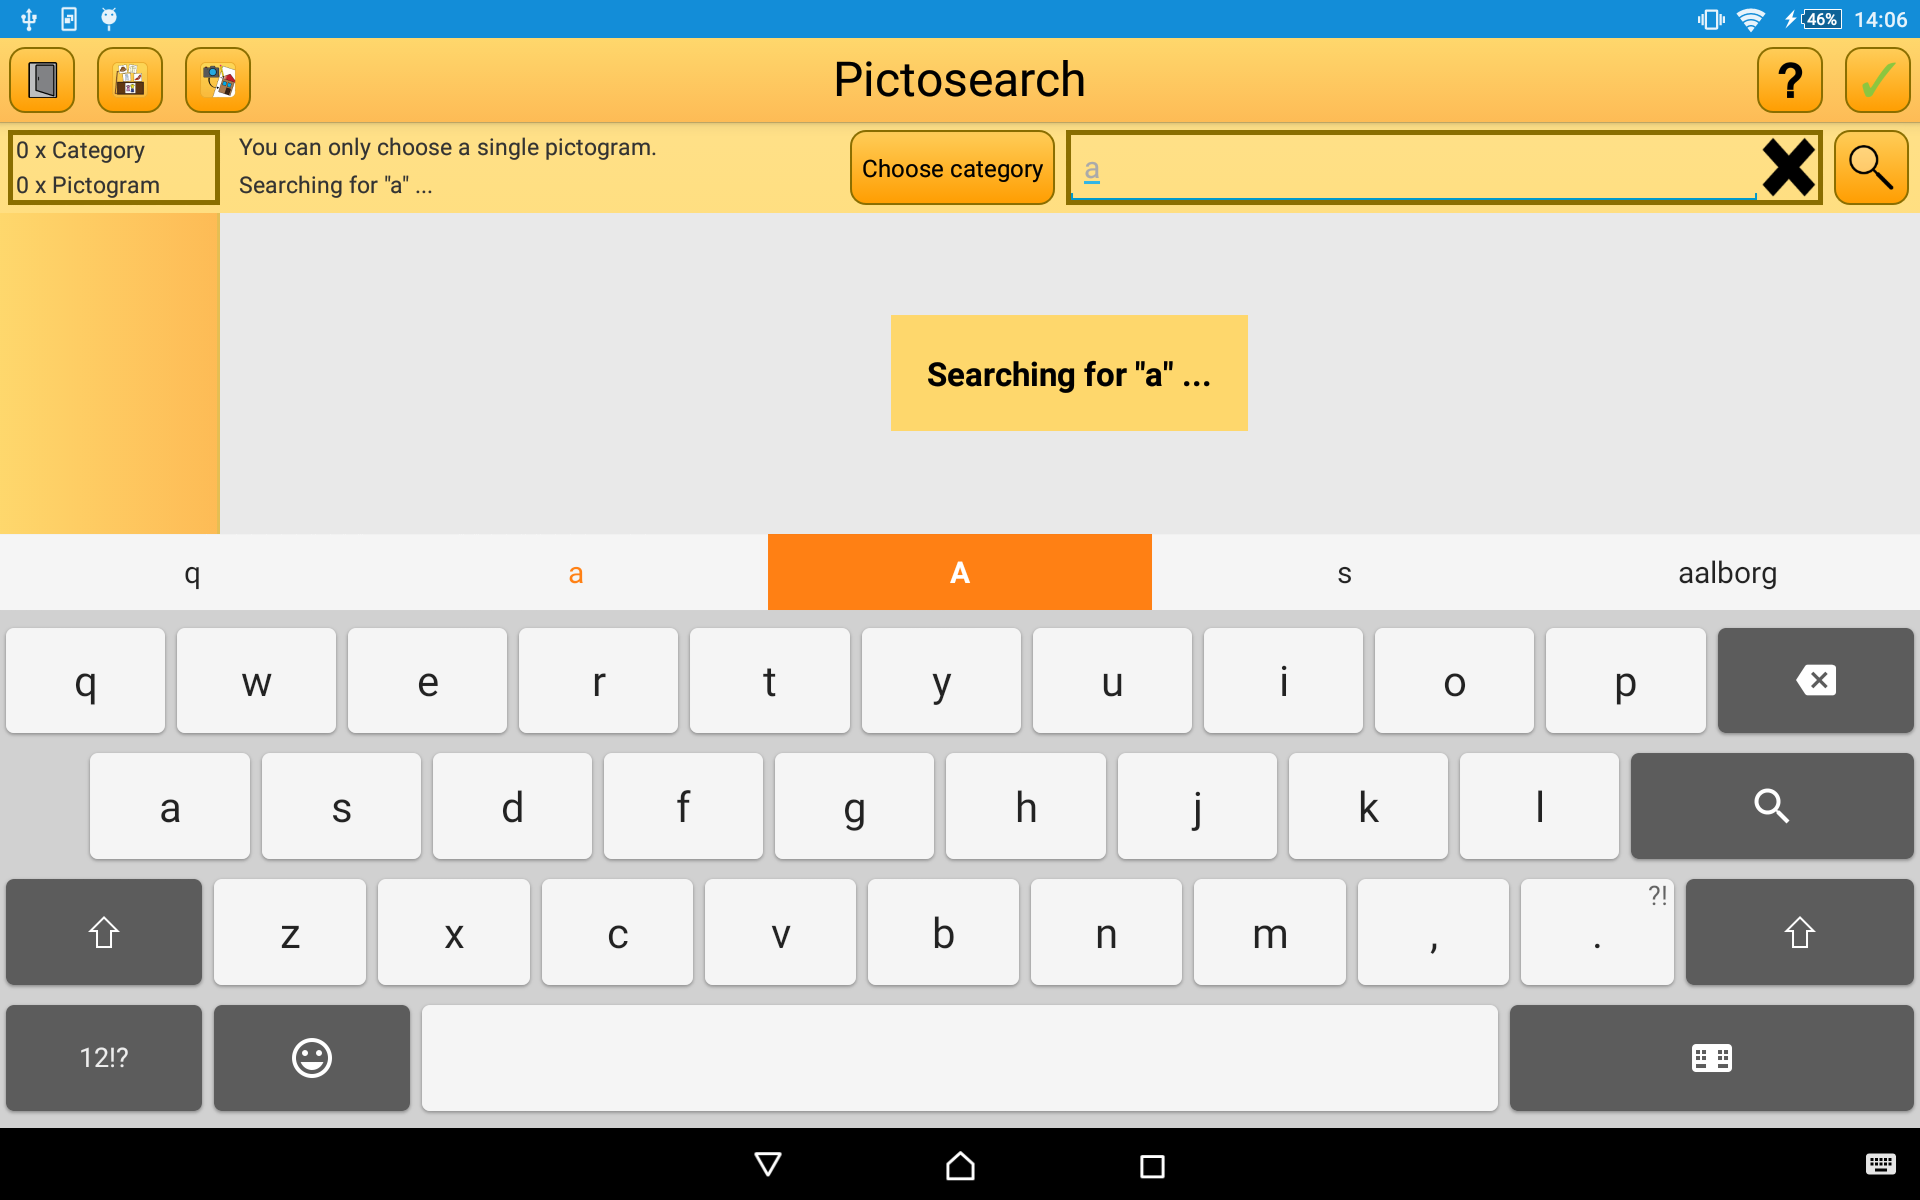
\includegraphics[width=0.8\textwidth]{figures/img/screenshots/new_dialog.png}
    \caption{Screenshot of the new search information, while searching.}\label{fig:screenshot_newsearch}
\end{figure}

This means that there is near instantaneous feedback for the user, which might give the feeling that the application is reacting to whatever the user is doing, and it might no longer feel to users like nothing is happening.
Previously the user would be waiting forever if he thought a search would be performed, when text was entered into the search--field, such as Google does. 
The new approach hereby provides search feedback significantly closer to the aforementioned 4 second limit.
Actually, the query which results in the largest amount of pictograms is a search for the character \enquote{s}, it returns 1932 pictograms and takes approximately 4 seconds on the relatively slow Lenovo tablet provided by the University --- as this is the worst case regarding search time, the average use case will always be faster than 4 seconds. 

The search button can still be used, and will bring up the old search spinner as usually, this is done so that \enquote{refreshing} a search result will provide feedback. 
Moreover the button has been moved from the middle of the display to the right side of the display as can be seen on \myref{fig:screenshot_newstartup}. 
This is a better fit as it resembles other common search engines such as Google Search, and it is also the recommended way to display a search-field according to the Niels Norman Group\footnote{https://www.nngroup.com/articles/magnifying-glass-icon/}.
Furthermore according to the principles of Constantine and Lockwood, structuring the interface is important such that it is for example recognisable: 

\begin{displayquote}
\textit{Organize the user interface purposefully, in meaningful and useful ways based on clear, consistent models that are apparent and recognizable to users, putting related things together and separating unrelated things, differentiating dissimilar things and making similar things resemble one
another.\cite[p.~51]{DESIGNBOOK}.}
\end{displayquote}
\noindent
Therefore using a familiar position of the button is a better fit than placing it in the middle of the screen as in the current version.

Another thing we noticed was that the clear search field button was visible all the time even though no text was in the search field.
This has been removed and it is now only visible when there is text in the search field i.e. when the actoion is available, as can be seen on \myref{fig:screenshot_newstartup} and it it still there on \myref{fig:screenshot_newsearch}.
This has been done because of another design pricinple by Constantine and Lockwood: 

\begin{displayquote}
\textit{Keep all needed options and materials for a given task visible without distracting the user with extraneous or redundant information \cite[p.~55]{DESIGNBOOK}.}
\end{displayquote}

\begin{figure}[h]
    \centering
    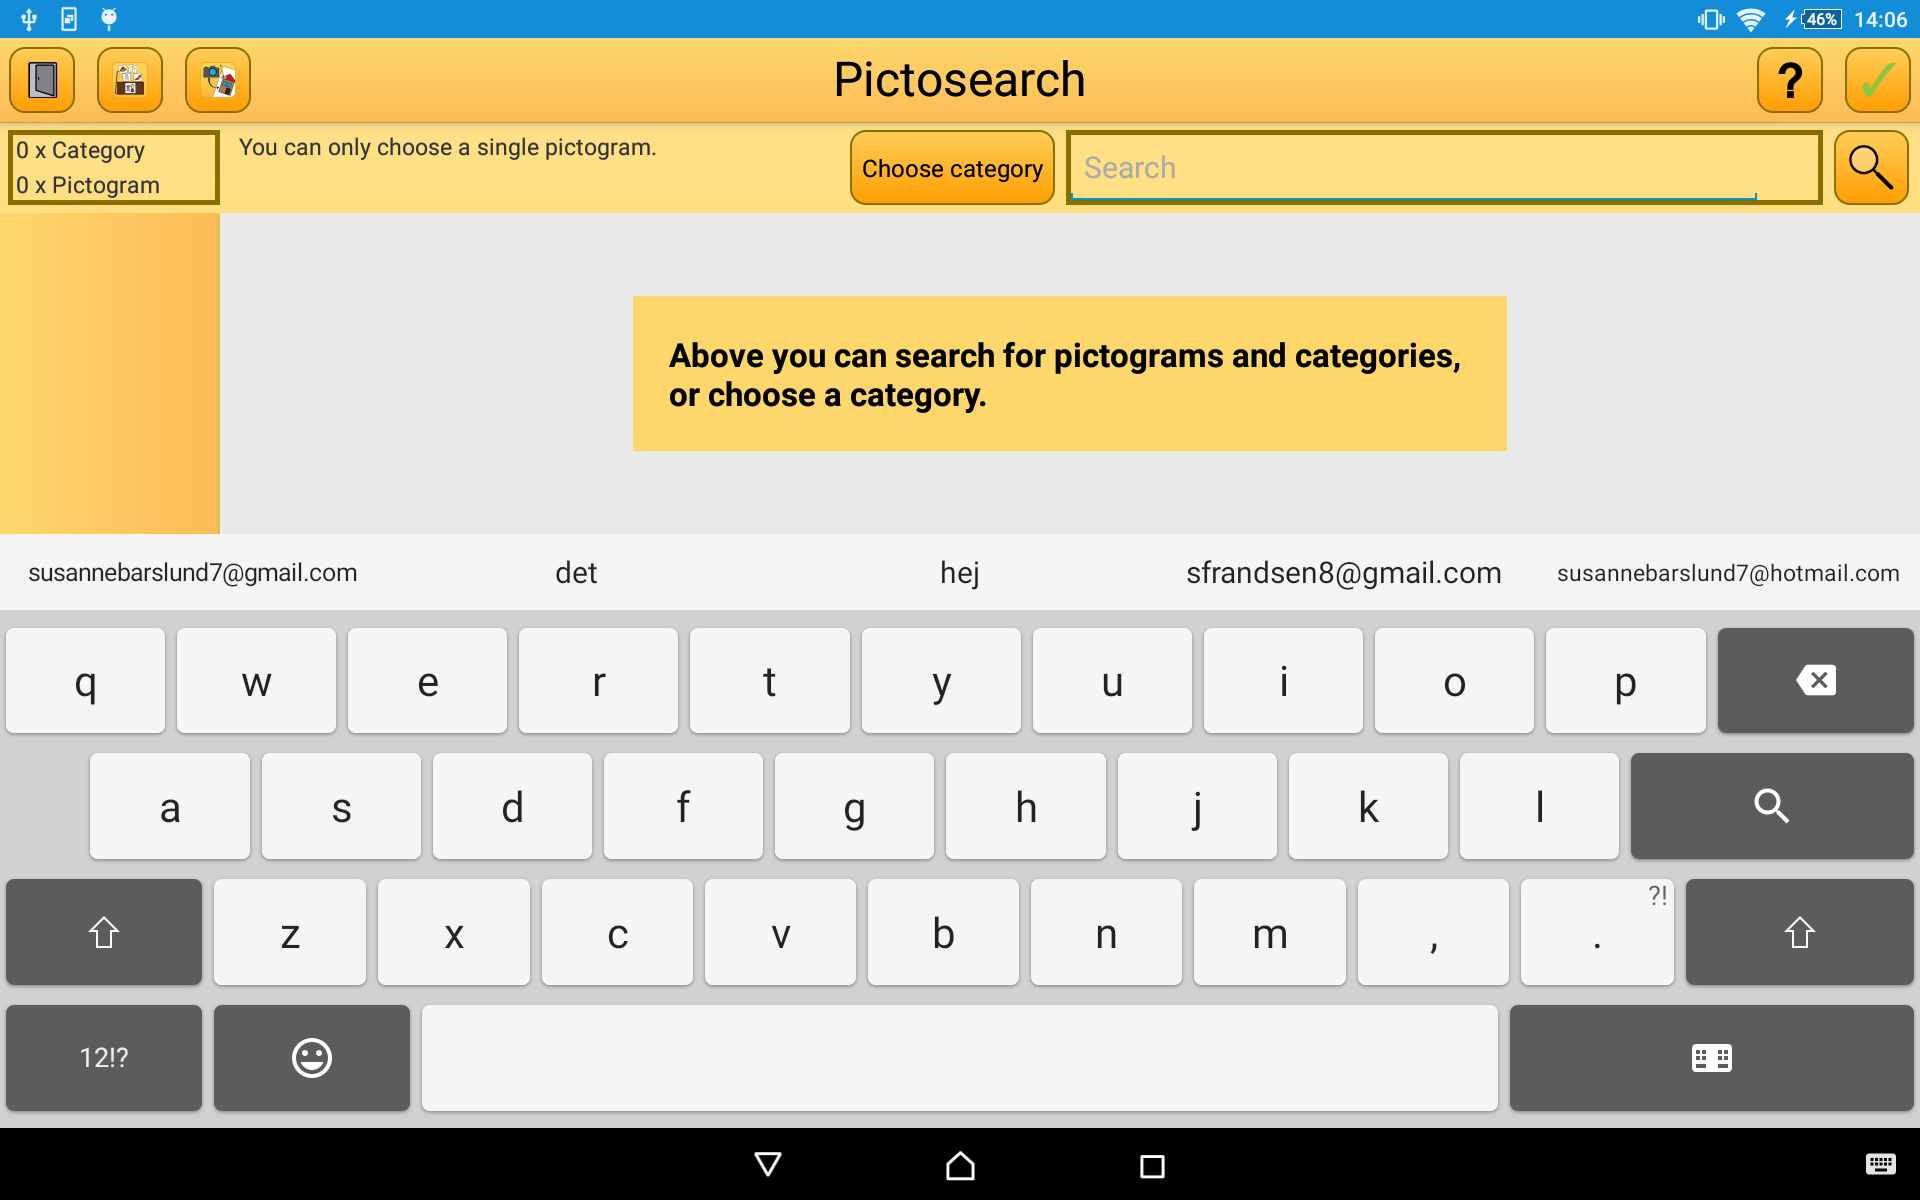
\includegraphics[width=0.8\textwidth]{figures/img/screenshots/new_startup.png}
    \caption{Screenshot of the new initial view in PictoSearch.}\label{fig:screenshot_newstartup}
\end{figure}


\section{dk.giraf.lib Breaks Gradle Build}
\todo[inline]{Nu har vi to rimelig forskellige beskrivelser af hvordan en task er løst, hvilken en vil vi benytte fremadrette? - M}
